\chapter{FUTURE WORK WITH DATA ASSIMILATION AND MACHINE LEARNING}
\label{chap:satfx}



\section{Satellite Image Forecasts}

\Cref{chap:satoi} and \cref{app:satoi} present a way in which a
nowcast of irradiance can be improved using data assimilation
techniques.
Naturally, we want to extend this nowcast into a proper forecast
initially using the technique of cloud motion vectors that produced
forecasts in \cref{chap:network} and \cref{app:network}.
More complicated dynamics other than advection such as cloud formation
and dissipation may be incorporated.
Eventually, a full numerical weather model may be required to capture
the dynamics of the system with the desired accuracy.


With a forecast model, it is natural to extend optimal interpolation
to the well known Kalman filter where a forecast of the state is
produced and constantly updated with new information.
This has the added benefit of retaining information from all previous
steps.
Errors will be present in an estimation of the cloud velocity field,
thus we will use an ensemble Kalman filter with an ensemble of
velocity fields.
An additional challenge will be integrating two types of observations
into the state of the sytem: new observations from ground sensors and
new satellite images.


In addition to introducing the forecast model and Kalman filter, we
will also explore extending the area of analysis and the number of
observations used.
\Cref{fig:allsensors} shows the locations of roughly 300 sensors that
may provide useful information to this data assimilation problem.
Some sensors such as the SURFRAD and NREL MIDC sites are regularly
maintained, calibrated, and report high resolution data.
Other sites such as those in the RAWS network provide hourly
irradiance values and may lack routine maintainence.

\begin{figure}
\centering
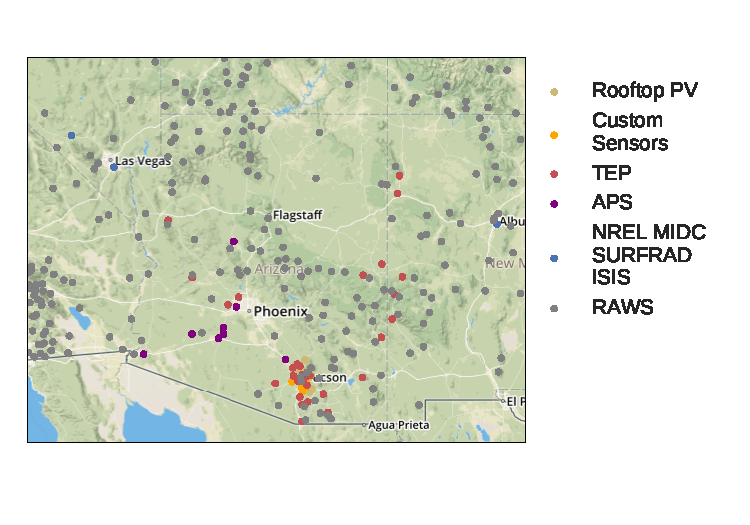
\includegraphics[width=\textwidth]{figs/azmap.pdf}
\vspace{-3em}
\caption[Map of all available irradiance sensors]{Map of all currently
available irradiance sensors near Arizona. These sensors come from a
number of networks with varying quality and time resolutions.}
\label{fig:allsensors}
\end{figure}

With the launch of GOES-16 a number of groups are developing products
and algorithms that make use of the new Advanced Baseline Imager
(ABI) and will provide better background state estimates.
The new ABI will image the continental US every five minutes with 16
spectral bands and resolutions as high as 0.5 km for the 0.64 $\mu$m
visible band.
Pictures of a comparison of the new GOES-16 and the current GOES-13
visible images in \cref{fig:goes_comp} and of a detailed image over
California in \cref{fig:goes_cal} show the impressive capabilities of
the instrument.

\begin{figure}[t]
\centering
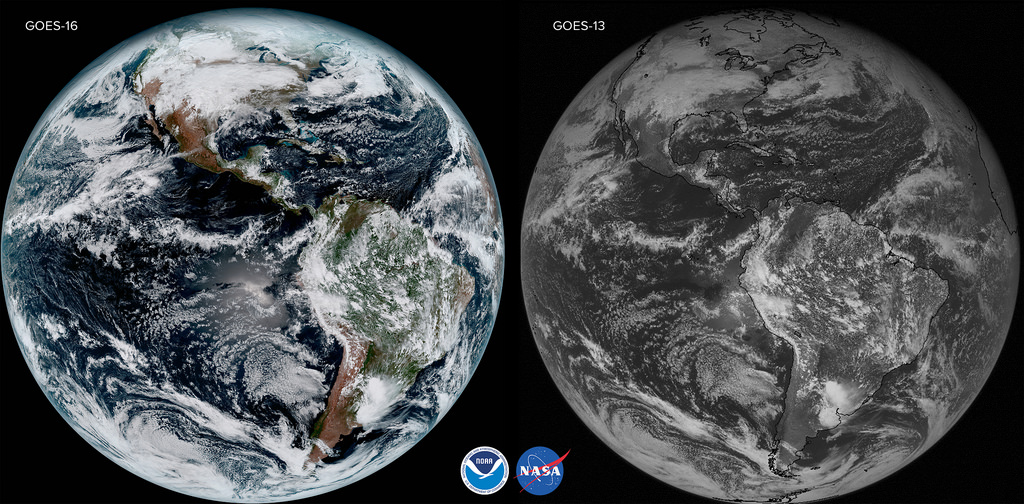
\includegraphics[width=\textwidth]{figs/goes_comp.jpg}
\caption[Comparison of visible images from the current and future
GOES]{A comparison of visible images created from the visible channels
of the new GOES-16 satellite and the previous generation
GOES-13. GOES-13 has only a single visible channel while GOES-16 has
three. Image courtesy of NOAA.}
\label{fig:goes_comp}
\end{figure}

\begin{figure}[h]
\centering
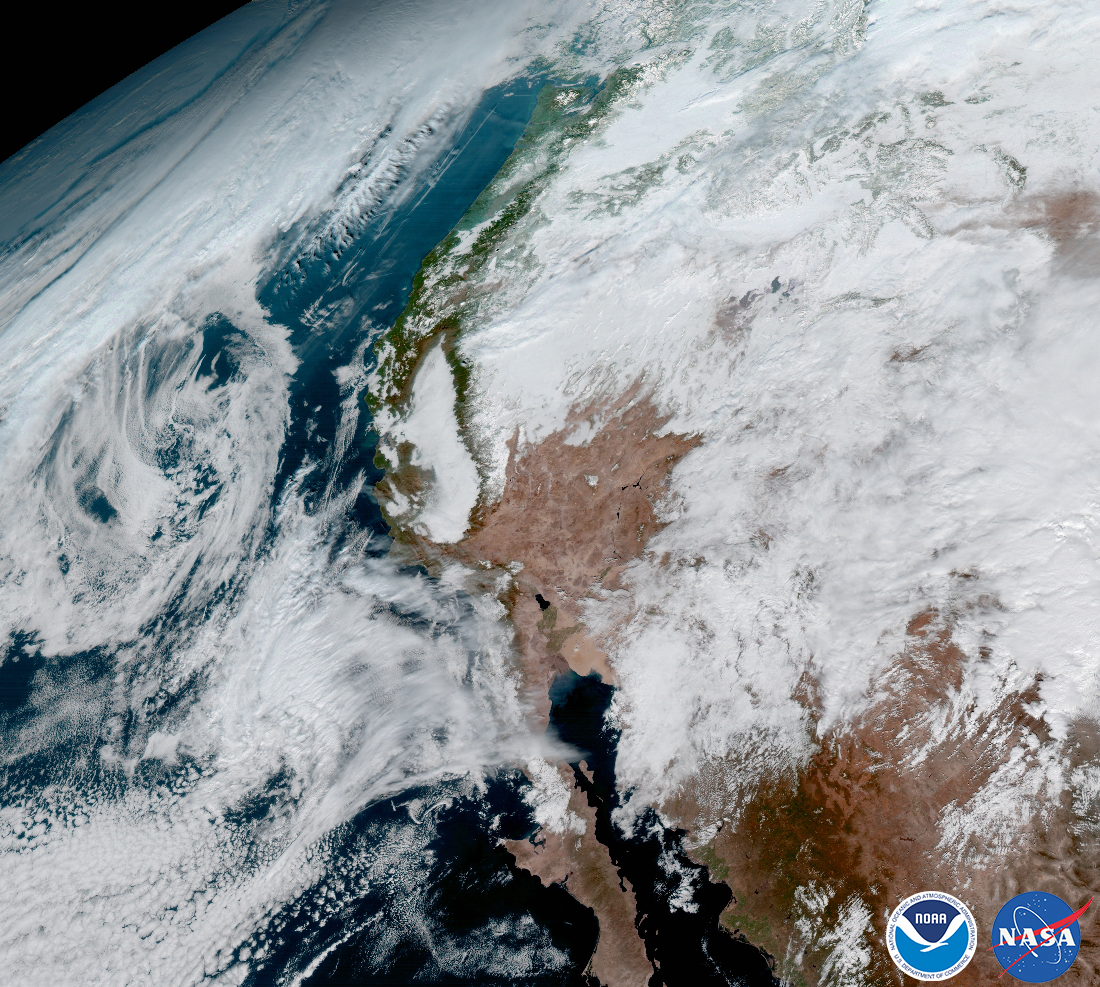
\includegraphics[width=0.8\textwidth]{figs/goes_cal.jpg}
\caption[An visible image of the western US from GOES-16]{A visible
image of the western US from the new GOES-16 satellite. The improved
resolution and spectral bands will improve satellite derived
irradiance estimates compared to the current generation of
satellite. Image courtesy of NOAA.}
\label{fig:goes_cal}
\end{figure}

A forecast regenerated every 5 minutes for 5 minutes to 6 hours in
advance covering a $300 \times 300$ km area over the state of Arizona
with 0.5 km resolution satellite estimates and 300 sensors from a 50
member (or larger) ensemble is a computationally daunting task.
Initial research into the local ensemble transform Kalman filter to
reduce the computational demands is promissing \citep{Hunt2007}.
Still, this problem will likely require use of a high performance
computing cluster and specialized compute hardware such as GPUs or
coprocessors.

\section{Intelligent Forecast Fusion}


%%% Local Variables:
%%% mode: latex
%%% TeX-master: "dissertation"
%%% End:
